\documentclass{article}

% if you need to pass options to natbib, use, e.g.:
%     \PassOptionsToPackage{numbers, compress}{natbib}
% before loading neurips_2020

% ready for submission
% \usepackage{neurips_2020}

% to compile a preprint version, e.g., for submission to arXiv, add add the
% [preprint] option:
%     \usepackage[preprint]{neurips_2020}

% to compile a camera-ready version, add the [final] option, e.g.:
     \usepackage[final]{neurips_2020}

% to avoid loading the natbib package, add option nonatbib:
%     \usepackage[nonatbib]{neurips_2020}

\usepackage[utf8]{inputenc} % allow utf-8 input
\usepackage[T1]{fontenc}    % use 8-bit T1 fonts
\usepackage{hyperref}       % hyperlinks
\usepackage{url}            % simple URL typesetting
\usepackage{booktabs}       % professional-quality tables
\usepackage{amsfonts}       % blackboard math symbols
\usepackage{nicefrac}       % compact symbols for 1/2, etc.
\usepackage{microtype}      % microtypography
\usepackage{graphicx}
\usepackage{float}

\title{AI Project 1: Drug Molecular Toxicity Prediction}

% The \author macro works with any number of authors. There are two commands
% used to separate the names and addresses of multiple authors: \And and \AND.
%
% Using \And between authors leaves it to LaTeX to determine where to break the
% lines. Using \AND forces a line break at that point. So, if LaTeX puts 3 of 4
% authors names on the first line, and the last on the second line, try using
% \AND instead of \And before the third author name.

\author{
MATSUNAGA TAKEHIRO \\
518030990028\\
Department of Computer Science\\
Shanghai Jiao Tong University\\
\texttt{matsunagatakehiro@sjtu.edu.cn} \\
}


\begin{document}

\maketitle

\begin{abstract}
 I develop some models to solve a problem whether a chemical is toxic or not. In this project I use residual net(ResNet), long short-term memory(LSTM) and a complex CNN based on LeNet-5. Through several experiment I found that the complex neural network is most accurate among these model.
\end{abstract}

\section{Introduction}
This project is the group project of CS410 Artificial Intelligence 2020 Fall in Shanghai Jiao Tong University named Drug Molecular Toxicity Prediction. The main purpose is to use a neural network model taking chemical structure as input, to output the prediction of whether it is toxic. In this project I use one hot format of SMILE structure which is processed from original chemical structure. The one hot format of SMILES is a 2D {0,1} matrix, where each column represents a symbol in the SMILES notation of the current molecule, and each row is one ASCII character appeared in the dataset’s SMILES dictionary.
% The authors develop two different neural network models, which are Deep Fully Connected Neural Networks with Merge-and-Run Mappings(DMRNets) and LSTM in their attempts to achieve this goal.

\section{Evironment}
In this project, TensorFlow-gpu 1.15.0 is used as deep learning library, Pandas is used to input data and Numpy is used through mathmatical calculation.

\section{Methods}
\subsection{Complex Convolutional Neural Networks}
Based on LeNet-5 which is given in the demo, I optimize that model by using batch normalization, droupout and so on. 

\subsubsection{LeNet-5}
LeNet-5 is a simple but usefull CNN which is widely used in image processing. The original LeNet-5 consists of seven layers: 2 convolution layer, 2 pooling layer and 3 full connection layer. The input data will first processed by Layer 1 convolution, that has 5$\times$5 kernel. Through the convolution it will increase the data channel. The pooling is use to reduce its size, and outstand feature value in pooling kernel. When the size is small enough--in LeNet-5 run the function after 2 convolution and pooling-- model run the full connection and shrink node to label size by using 3 layers. The Figure 1 show the structure of LeNet-5.
\begin{figure}[h]
  \centering
  \fbox{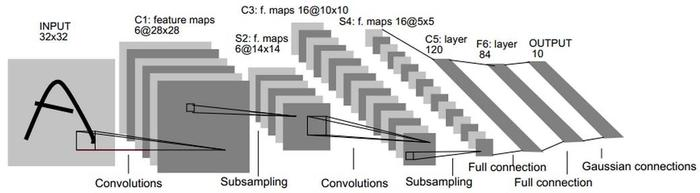
\includegraphics[width=14cm, height=4cm]{LeNet-5.png}}
  \caption{Structure of LeNet-5}
\end{figure} 

\subsubsection{Complex CNN}
The size of input data of one hot format is (?, 73, 398), which means each size of one chemical matrix is 73$\times$398. 


\subsubsection{Performance}
Small datasets MAP@10: 
Whole datasets MAP@10: 

\subsection{CNN + LSTM}
\subsubsection{Model Overview}
Long short-term memory(LSTM) is a type of recurrent neural network (RNN) architecture,which is one of the most useful RNN.  Before LSTM, let's first talk about RNN, the structure of a typical RNN is shown in Figure x. As brain can understand articles based on knowledge that people have learnt before, some parameters in RNN can be derived from forward node, this was what traditional neural networks could not achieve. Traditional RNN could not store what it learned from forward node for a dragged time period, since every cell of RNN will process both input and derived information in activation function, but LSTM solved this problem.


A common LSTM unit is composed of a cell and 3 gates. The cell stores values over time intervals as cell states, and the 3 gates’ main job is to regulate the flow of information into and out of the cell. Specifically, forget gate decides which information to forget, input gate decides to update which value of cell states and update cell states, and at last, the output gate output filtered cell states. To put it in an abstract high-level view, what LSTM do is using past context as reference to predict the output.Beside forward outputs, another data are derived from forward nodes in LSTM network. The increasing data will only interact with a few data that processed in cell, which means it will keep the knowledge that it learned for a long time.

\begin{figure}[h]
  \centering
  \fbox{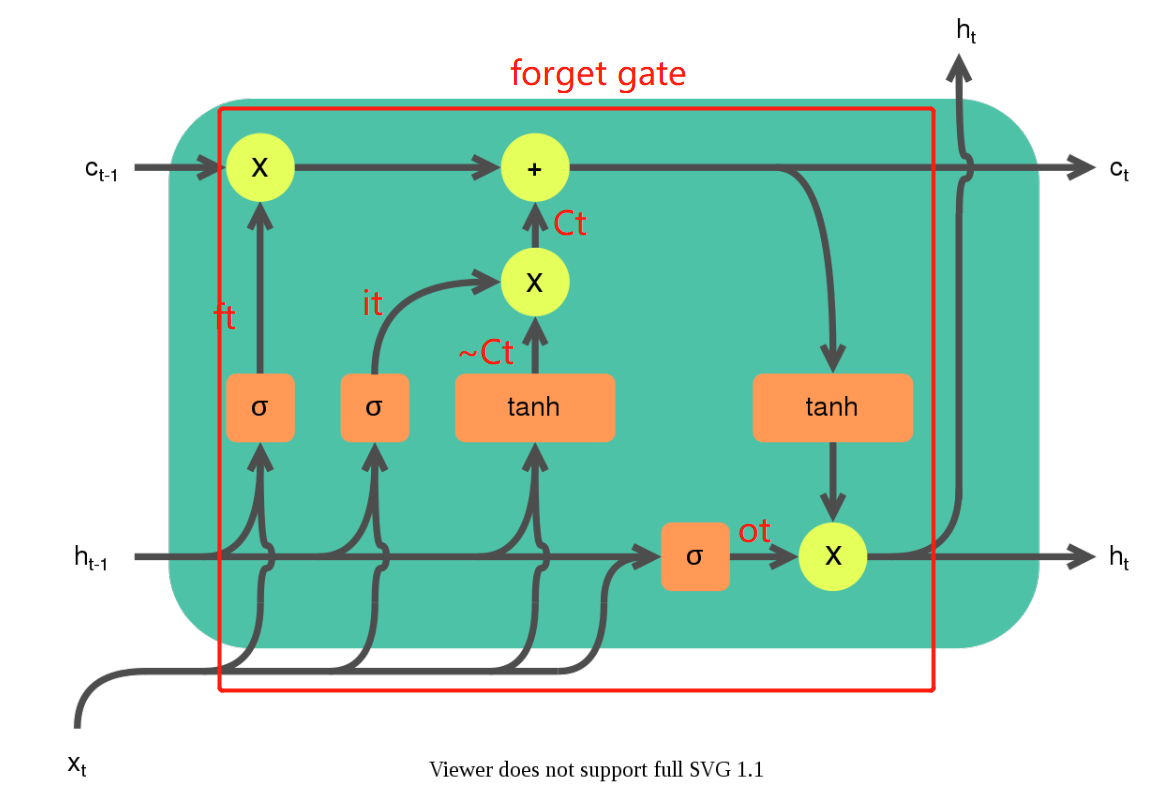
\includegraphics[width=14cm, height=9cm]{lstm.png}}
  \caption{Structure of LSTM Cell}
\end{figure} 


Here are each step in the forget gate of LSTM cell:
\begin{itemize}
\item step1: $f_t = \sigma(W_f[h_{t-1}, x_t] + b_f)$
\item step2: $i_t = \sigma(W_i[h_{t-1}, x_t] + b_i)$,  $\widetilde{C} = tanh(W_C[h_{t-1}, xt] + b_C)$
\item step3: $o_t=\sigma(W_o[h_{t-1}, x_t] + b_o)$
\item step4: $C_t = f_t*C_{t-1} + i_t*\widetilde{C}$
\item step5: $h_t=o_t*tanh(C_t)$
\end{itemize}

\subsubsection{Contribute idea}
The reason why I use CNN first is that the input size is too huge for my computer to caluculate directly. So CNN and pooling is necessary for reduce the size. When passing the CNN layer, the size of each piece of data is $18*50*32$. So I can run the processed input on LSTM, which can keep some forward information.



\subsubsection{Performance}
Small datasets MAP@10: 
Whole datasets MAP@10: 

\subsection{Bidirectional Long short-term memory (biLSTM)}
\subsubsection{Model Overview}
biLSTM is a variant of LSTM, biLSTM train 2 instead of 1 LSTMs on 1 input sequence, the first on the input sequence, and the second on a reversed copy of the input sequence. In other words, it connects two hidden layers of opposite directions to the same output, this generally provide additional context to the network, thus results in better training results. for more information please refer to the original article[4]. The model structure is shown in Figure 6.


In our project, we train two features in each biLSTM, then merge them together. Through full connection layer and leaky relu activation, the network will give final results. The model structure detail is in Figure (x).

The model first extend mean\_RGB features to 1024. Processing the data by using batch normalization and reshape in order to run bidirectional LSTM. Then model use dropout to make some noise. The process of the other feature is as same as RGB feature. When two features have done biLSTM, model concatenate them and full connect them using leaky relu. 

\subsubsection{Performance}
Small datasets MAP@10: 
Whole datasets MAP@10: 


\section{Experiments and Analysis}
\subsection{Training}
We wanted to use cloud platforms to train our model, but most of them needs payment, and we don't have the fund for that, Google Cloud Platform offers 1 month free trial, but to get the free trial we need to register with credit card, which unfortunately we don't possess, at the end of the day we need to train the model using our local machines. Limited by the performance of our local machines, we could only use a small subset of the datasets for training, in this case, we use the first 200 training shards (train0000.tfrecord~train0199.tfrecord) and the first 100 validation shards (validate0000.tfrecord~validate0099.tfrecord) as our training datasets. Figure 6 and 7 shows the graph of training curve of the LSTM and biLSTM models. As shown in the figures, both models converged at around $0.75$, with biLSTM having a slightly better performance.



\subsection{Comparison and Analysis of Performance}
\begin{table} [H]
  \caption{Performance of different models}
  \label{table 1}
  \centering
  \begin{tabular}{llll}
    \toprule
    Model     & 200 train MAP@10     & 100 validation MAP@10 & All datasets MAP@10 \\
    \midrule 
DMRNets & 0  & 0   &0  \\
LSTM & 0  & 0 & 0.759     \\
biLSTM     & 0 & 0 & 0.763      \\
    \bottomrule
  \end{tabular}
\end{table}
The performances of 3 models are listed in Table \ref{table 1}, as we could see, the MAP@10 for the first 200 training shards and 100 validation shards are always higher than the MAP@10 for the whole datasets, the reason is obvious as we use the first 200 training shards and 100 validation shards as training datasets which leads to possible overfitting. However, we consider that the LSTM and biLSTM's performance of around 0.75 to 0.76 for the whole datasets as satisfactory, since we only use an extremely small subset to train them. We hypothesize that if we use larger datasets for training, the model would lead to more satisfactory results, too bad that we don't have the computing power to prove this hypothesis.



\section{Conclusion}
Based on the experiments, we conclude that the xxx model has a superior performance over the other models we used.


\section*{References}

References follow the acknowledgments. Use unnumbered first-level heading for
the references. Any choice of citation style is acceptable as long as you are
consistent. It is permissible to reduce the font size to \verb+small+ (9 point)
when listing the references.
{\bf Note that the Reference section does not count towards the eight pages of content that are allowed.}
\medskip

\small

[1] Kaiming He, Xiangyu Zhang, Shaoqing Ren, Jian Sun. Deep Residual Learning for Image Recognition.

[2] Liming Zhao, Mingjie Li, Depu Meng, Xi Li, Zhaoxiang Zhang. Deep Convolutional Neural Networks with Merge-and-Run Mappings.

[3] Sepp Hochreiter. Long Short-Term Memory. 

[4] Alex Graves, Jürgen Schmidhuber. Framewise phoneme classification with bidirectional LSTM and other neural network architectures. 
\end{document}
